\chapter{Конструкторская часть}
В данном разделе представлены схемы алгоритмов, описанных в
аналитическом разделе, а также будет подсчитана их трудоемкость.
\section{Трудоемкость алгоритмов}

\subsection{Модель вычислений}

Для последующего вычисления трудоемкости введём модель вычислений:
\begin{enumerate}
	\item Трудоемкость базовых операций:
	Пусть операции из (\ref{for:opers1}) имеют единичную трудоемкость.
	\begin{equation}
	\label{for:opers1}
	+, -, =, ==, !=, <, >, <=, >=, [], +=, -=, <<, >>
	\end{equation}
	
	Пусть операции из (\ref{for:opers2}) имеют трудоемкость 2.
	\begin{equation}
	\label{for:opers2}
	/, *, \%
	\end{equation}
		
	\item Трудоемкость условного оператора ``if условие then A else B'' рассчитывается, как (\ref{for:if}).
	\begin{equation}
	\label{for:if}
	f_{if} = f_{\text{условия}} +
	\begin{cases}
	f_A, & \text{если условие выполняется,}\\
	f_B, & \text{иначе.}
	\end{cases}
	\end{equation}

	\item Трудоемкость цикла рассчитывается по C-подобной модели, то есть ``for (i = 0; i < N; i += 1)'', как (\ref{for:for}).
	\begin{equation}
	\label{for:for}
	f_{for} = f_{\text{инициализации}} + f_{\text{сравнения}} + N(f_{\text{тела}} + f_{\text{инкремента}} + f_{\text{сравнения}})
	\end{equation}

	\item Трудоемкость вызова функции равна 0.

	\item Трудоемкость внутреннего цикла с переменным пределом рассчитывается, как (\ref{eq:var_cycle}).

	\begin{equation}
		\label{eq:var_cycle}
		f = f_{\text{служебное}} + Q_{\text{сравнения}} \cdot f_{\text{на 1 сравнение}}
	\end{equation}
	
	$f_{\text{служебное}}$ -- затраты на содержание внешнего цикла, инициализацию и стартовое сравнение вложенного 
	цикла.
	
	$Q_{\text{сравнения}}$ -- количество сравнений. 
	
	$f_{\text{на 1 сравнение}}$ -- затраты на содержание 1 сравнения, то есть условия инкремента и сравнения вложенного цикла.
\end{enumerate}


\subsection{Алгоритм сортировки пузырьком}

Размер исходного массива принимается за N. 

Для рассчета трудоемкости внутреннего цикла с переменным пределом используется формула \ref{eq:var_cycle}.

$f_{\text{на 1 сравнение}}$ определяется выражением \ref{eq:bubble-fper1cmp}.
\begin{equation}
	\label{eq:bubble-fper1cmp}
	f_{\text{на 1 сравнение}} = 7 + \begin{cases}
	0, & \text{в лучшем случае}\\
	9, & \text{в худшем случае}
	\end{cases}
\end{equation}

$Q_{\text{сравнения}}$ определяется выражением \ref{eq:bubble-qcmp}.
\begin{equation}
	\label{eq:bubble-qcmp}
	Q_{\text{сравнения}} = \frac{N(N-1)}{2} = \frac{N^{2}}{2} - \frac{N}{2}
\end{equation}

$f_{\text{служебное}}$ определяется выражением \ref{eq:bubble-fserve}.
\begin{equation}
	\label{eq:bubble-fserve}
	f_{\text{служебное}} = 3 + (N - 1) \cdot (3 + 3) = 6N - 3
\end{equation}


Трудоемкость в лучшем случае (отсортированный массив) описывается выражением \ref{eq:bubble-best}
\begin{equation}
	\label{eq:bubble-best}
	f_{\text{bubble-best}} = (6N - 3) + (\frac{N^{2}}{2} - \frac{N}{2})\cdot7 = 4.5N^{2}+2.5N-3 \approx 4.5N^{2}
\end{equation}


Трудоемкость в худшем случае (отсортированный в обратном порядке массив) описывается выражением \ref{eq:bubble-worst} 
\begin{equation}
	\label{eq:bubble-worst}
	f_{\text{bubble-worst}} = (6N - 3) + (\frac{N^{2}}{2} - \frac{N}{2})\cdot16 = 8N^{2}-2N-3 \approx 8N^{2}
\end{equation}

\subsection{Алгоритм сортировки выбором}

Размер исходного массива принимается за N. 

Для рассчета трудоемкости внутреннего цикла с переменным пределом также, как и для алгоритма сортировки
пузырьком, используется формула \ref{eq:var_cycle}.

$f_{\text{на 1 сравнение}}$ определяется выражением \ref{eq:select-fper1cmp}.
\begin{equation}
	\label{eq:select-fper1cmp}
	f_{\text{на 1 сравнение}} = 5 + \begin{cases}
	0, & \text{в лучшем случае}\\
	1, & \text{в худшем случае}
	\end{cases}
\end{equation}

$Q_{\text{сравнения}}$ определяется выражением \ref{eq:select-qcmp}.
\begin{equation}
	\label{eq:select-qcmp}
	Q_{\text{сравнения}} = \frac{N(N-1)}{2} = \frac{N^{2}}{2} - \frac{N}{2}
\end{equation}

$f_{\text{служебное}}$ определяется выражением \ref{eq:select-fserve}.
\begin{equation}
	\label{eq:select-fserve}
	f_{\text{служебное}} = 3 + (N - 1) \cdot (3 + 4) = 7N - 4
\end{equation}

Трудоемкость в лучшем случае (отсортированный массив) описывается выражением \ref{eq:select-best}
\begin{equation}
	\label{eq:select-best}
	f_{\text{select-best}} = (7N-4) + (\frac{N^{2}}{2} - \frac{N}{2})\cdot5 = 2.5N^{2}+4.5N-4 \approx 2.5N^{2}
\end{equation}

Трудоемкость в худшем случае (отсортированный в обратном порядке массив) описывается выражением \ref{eq:select-worst} 
\begin{equation}
	\label{eq:select-worst}
	f_{\text{select-worst}} = (7N-4) + (\frac{N^{2}}{2} - \frac{N}{2})\cdot6 = 3N^{2}+4N-4 \approx 3N^{2}
\end{equation}
\newpage

\section{Схемы алгоритмов}

На рисунке \ref{scheme:bubble} представлена схема алгоритма сортировки пузырьком.
\begin{figure}[!htb]
	\centering
	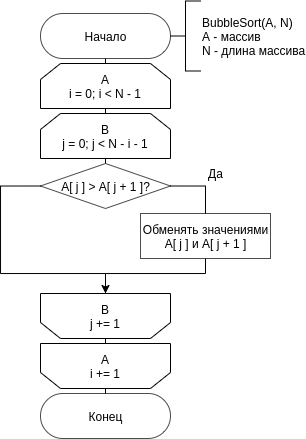
\includegraphics[scale=0.56]{schemes/bubble}
	\caption{Схема алгоритма сортировки пузырьком}
	\label{scheme:bubble}
\end{figure}

На рисунке \ref{scheme:select} представлена схема алгоритма сортировки выбором.
\begin{figure}[!htb]
	\centering
	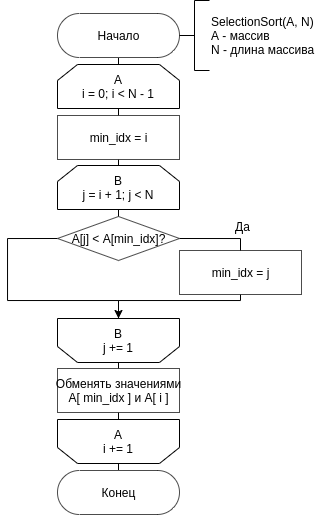
\includegraphics[scale=0.56]{schemes/select}
	\caption{Схема алгоритма сортировки выбором}
	\label{scheme:select}
\end{figure}

На рисунке \ref{scheme:insert} представлена схема алгоритма сортировки вставками.
\begin{figure}[!htb]
	\centering
	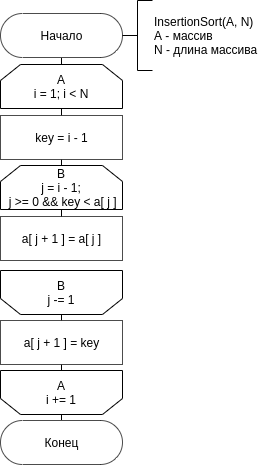
\includegraphics[scale=0.56]{schemes/insert}
	\caption{Схема алгоритма сортировки выбором}
	\label{scheme:insert}
\end{figure}
% \newpage

\section{Вывод}
На основе теоретических данных, полученных из аналитического раздела, 
были построены схемы трех алгоритмов сортировки. На основе введенной 
модели вычислений оценена трудоемкость алгоритма сортировки пузрьком 
и алгоритма сортировки выбором в луч­шем и худшем случаях.

Из преведнных оценок трудоемкостей алгоритмов следует, что алгорим 
сортировки выбором имеет меньшую трудоемкость, чем алгоритм сортировки
пузырьком. Для лучшего и худшего случаев соответственно в $1.8$ и $2.7$ раза.
